%%%%%%%%%%%%
%% Please rename this main.tex file and the output PDF to
%% [lastname_firstname_graduationyear]
%% before submission.
%%
%% This .tex file is for use with BibLaTeX. Please use
%% main-bibtex.tex instead if you prefer BibTeX.
%%%%%%%%%%%%

\documentclass[12pt]{caltech_thesis}
\usepackage[hyphens]{url}
\usepackage{lipsum}
\usepackage{graphicx}
\usepackage{subcaption}
\usepackage{todonotes}
\usepackage{physics}
\usepackage{booktabs}
\usepackage{tikz}
\usepackage{pgf}

%% Tentative: newtx for better-looking Times
\usepackage[utf8]{inputenc}
\usepackage[T1]{fontenc}
\usepackage{newtxtext,newtxmath}
% Must use biblatex to produce the Published Contents and Contributions, per-chapter bibliography (if desired), etc.
\usepackage[
    backend=biber,natbib,
    % IMPORTANT: load a style suitable for your discipline
    style=nature
]{biblatex}
\usepackage{nomencl}


\makenomenclature
%% This code creates the groups
% -----------------------------------------
\usepackage{etoolbox}
\renewcommand\nomgroup[1]{%
  \item[\bfseries
  \ifstrequal{#1}{M}{Molecular orbital basis}{%
  \ifstrequal{#1}{N}{Number sets}{%
  \ifstrequal{#1}{O}{Other symbols}{}}}%
]}
% -----------------------------------------

\usepackage{listings} % Required for insertion of code
\usepackage{xcolor} % Required for custom colors

% Define custom colors
\definecolor{codegreen}{rgb}{0,0.6,0}
\definecolor{codegray}{rgb}{0.5,0.5,0.5}
\definecolor{codepurple}{rgb}{0.58,0,0.82}
\definecolor{backcolour}{rgb}{0.95,0.95,0.92}

% Setup the style for code listings
\lstdefinestyle{mystyle}{
    backgroundcolor=\color{backcolour},   
    commentstyle=\color{codegreen},
    keywordstyle=\color{magenta},
    numberstyle=\tiny\color{codegray},
    stringstyle=\color{codepurple},
    basicstyle=\ttfamily\footnotesize,
    breakatwhitespace=false,         
    breaklines=true,                 
    captionpos=b,                    
    keepspaces=true,                 
    numbers=left,                    
    numbersep=5pt,                  
    showspaces=false,                
    showstringspaces=false,
    showtabs=false,                  
    tabsize=2
}

% Activate the style
\lstset{style=mystyle}
\usepackage{hyperref}
\usepackage{multirow}

% Name of your .bib file(s)
\addbibresource{examples.bib}
\addbibresource{ownpubs.bib}

\begin{document}

% Do remember to remove the square bracket!
\title{$G_0W_0$ for Molecules}
\author{Patryk Kozlowski}

\degreeaward{Bachelor of Science in Chemistry}                 % Degree to be awarded
\university{California Institute of Technology}    % Institution name
\address{Pasadena, California}                     % Institution address
\unilogo{caltech.png}                                 % Institution logo
\copyyear{2024}  % Year (of graduation) on diploma
\defenddate{[Exact Date]}          % Date of defense

\orcid{0009-0000-6402-4261}

%% IMPORTANT: Select ONE of the rights statement below.
\rightsstatement{All rights reserved}
% \rightsstatement{All rights reserved except where otherwise noted}
% \rightsstatement{Some rights reserved. This thesis is distributed under a [name license, e.g., ``Creative Commons Attribution-NonCommercial-ShareAlike License'']}

%%  If you'd like to remove the Caltech logo from your title page, simply remove the "[logo]" text from the maketitle command
\maketitle[logo]
%\maketitle

\begin{acknowledgements} 	 
   [Add acknowledgements here. If you do not wish to add any to your thesis, you may simply add a blank titled Acknowledgements page.]
\end{acknowledgements}

\begin{abstract}
   [This abstract must provide a succinct and informative condensation of your work. Candidates are welcome to prepare a lengthier abstract for inclusion in the dissertation, and provide a shorter one in the CaltechTHESIS record.]
\end{abstract}

%% Uncomment the `iknowhattodo' option to dismiss the instruction in the PDF.


\tableofcontents
\listoffigures
\listoftables
\printnomenclature

\mainmatter

\chapter{Nomenclature}
\label{chap:nomenclature}
\begin{tabular}{p{0.65\textwidth} p{0.8\textwidth}}
Symbol & Description \\
\hline
\(i,j,k,l\) & Occupied orbital indices \\
\(a,b,c,d\) & Virtual orbital indices \\
\(p,q,r,s\) & General MO indices \\
\(\mu,\nu,\lambda,\sigma\) & AO indices \\
\((pq|rs) = \int \int \psi_p^*(\mathbf{r}_1)\psi_q(\mathbf{r}_1)\frac{1}{r_{12}}\psi_r^*(\mathbf{r}_2)\psi_s(\mathbf{r}_2)d\mathbf{r}_1d\mathbf{r}_2\) & Two-electron spatial integrals\\
\((pq||rs) = (pq|rs) - (ps|rq)\) & Antisymmetrized two-electron integrals \\
\(\chi _p (\mathbf{x}) = \psi _p (\mathbf{r})\sigma (\mathbf{\omega })\) & Spin-orbital \\
\([pq|rs] = \int \int \chi_p^*(\mathbf{x}_1)\chi_q(\mathbf{x}_1)\frac{1}{r_{12}}\chi_r^*(\mathbf{x}_2)\chi_s(\mathbf{x}_2)d\mathbf{x}_1d\mathbf{x}_2\) & Two-electron spin integrals \\

\end{tabular}\\\\
All calculations have been done using the PySCF package.\autocite{sun_recent_2020} The code for this project can be found at \url{https://github.com/pkozlows/gw_senior_thesis/tree/master}.
\chapter{Motivation}
The formalism of many-body perturbation theory (MBPT) provides corrections to a mean-field description such as that given by Hartree-Fock or density functional theory (DFT). Hartree-Fock is not used much in practice because it is known to provide a weak treatment of electron correlation chiefly due to the fact that it only considers a single Slater determinant. DFT is often used for systems of large size, as it is fairly accurate and computationally cheap, scaling like $O(N^3)$, where $N$ is the system size. However, it treats electron correlation in an approximate way that is difficult to systematically improve. Specifically, its reliance on approximate functionals gives rise to the notorious self-interaction error; because one is using the electron density to determine the Coulomb repulsion between electrons, this means that one can have the electron interacting with its own contribution to the electron density. In practice, this can potentially lead to a variety of issues, including the underestimation of surface stability (overestimation of surface energies) relevant in surface science studies. \autocite{schimka_accurate_2010} \autocite{kozlowski_elucidating_2021} To remedy the problems with the mean field approximations, normally one would fall back onto the wave function-based MBPT, such as Moller-Plesset perturbation theory to 2nd order (MP2) and coupled cluster theory (CC). However, their computational scaling is steep, scaling like $O(N^5)$ and $O(N^6)$ or greater, respectively, which can make it difficult to simulate larger systems. \autocite{mcclain_gaussian-based_2017} To bridge the gap between the cheap mean-field methods and the expensive wave function-based MBPT, there has been an interest in applying Green's function MBPT methods, within the $GW$ approximation, to such systems, which has shown to give accurate corrections to various properties, such as band gaps, on top of a prior (DFT) mean-field calculation, at a moderate computational cost. \autocite{noauthor_frontiers_nodate} This is the motivation for my study of the $G_0W_0$ method, which traditionally scales like $O(N^4)$, within the framework of the $GW$ approximation.



\chapter{Theory}
We begin by writing out the time independent Schrödinger equation for the $N$-electron system
\begin{equation}
    \hat{H}\Psi =E\Psi 
\label{eqn:tise}
\end{equation}
with
\begin{equation}
\hat{H}=\sum_{i=1}^N\left(-\frac{1}{2} \nabla_i^2\right)-\sum_{i=1}^N \sum_{\alpha }\frac{Z_{\alpha }}{r_{i\alpha }}+\sum_{i<j}^N \frac{1}{r_{i j}} + C_{nn}.
\label{eqn:hamiltonian}
\end{equation}
An equation \ref{eqn:tise}, $\hat{H}$ is the Hamiltonian operator, $\Psi$ is the wave function, and $E$ is the energy of the system. As shown in equation \ref{eqn:hamiltonian}, the Hamiltonian operator consists of four terms: a kinetic energy term, in which a sum of the kinetic energy $-\frac{1}{2} \nabla_i^2$ of each electron is taken; a nuclear-electron attraction term, in which we have sums running over all of the electrons $i$ and all of the nuclei $\alpha$ with their separation denoted by $r_{i\alpha}$ and the nuclear charge denoted by $Z_{\alpha}$; an electron-electron repulsion term, in which we have a sum running over all pairs of electrons $i$ and $j$ with their separation denoted by $r_{ij}$; and a nuclear-nuclear repulsion term $C_{nn}$, which we have denoted as a constant since we are working in the Born-Oppenheimer approximation of all electrons moving in a fixed nuclear framework.
 The objective of many years of research in quantum chemistry has been solving for the electron-electron repulsion term, will we will call $V_{ee}$.
Now, I will introduce some of the mean field methods that have been classically used to tackle this problem at a cheap computational cost.
\section{Mean Field Methods}
\subsection{Hartree-Fock\autocite{szabo_modern_2012}}
\label{sec:hf}
The concept behind Hartree-Fock (HF) is that we can assign each electron a given orbital $\chi (\mathbf{r}, \sigma)$, where $\mathbf{r}$ is the spatial coordinate and $\sigma$ is the spin. Then, we take a Hartree product of these orbitals
\begin{equation}
    \Phi _{Hartree} = \chi _1(\mathbf{r}_1, \sigma_1) \chi _2(\mathbf{r}_2, \sigma_2) \cdots \chi _N(\mathbf{r}_N, \sigma_N).
\end{equation}
However, this is not antisymmetric with respect to the exchange of two electrons, so we need to enforce antisymmetry by taking a Slater determinant of these orbitals, denoting the antisymmetrization operator as $\hat{A}$,
\begin{equation}
    \Psi _{HF} = \hat{A} \prod_{i=1}^{N} \chi _i(\mathbf{r}_i, \sigma_i) .
\end{equation}
So we have arrived at the Hartree-Fock energy, which is defined as
\begin{equation}
    E_{HF} = \langle \Psi _{HF} | \hat{H} | \Psi _{HF} \rangle,
\end{equation}
where we have assumed the normalization $\langle \Psi _{HF} | \Psi _{HF} \rangle = 1$.
Now we seek to minimize this energy with respect to the constituent orbitals. This may be done by defining the Lagrangian
\begin{equation}
    \mathcal{L} = E_{HF} - \lambda \left( \langle \Psi _{HF} | \Psi _{HF} \rangle - 1 \right),
\end{equation}
where $\lambda$ is a Lagrange multiplier that enforces the normalization condition. We then take the functional derivative of the Lagrangian with respect to the orbitals and set it to zero to find the minimum of the energy
\begin{equation}
    \frac{\delta \mathcal{L}}{\delta \chi _i} = 0.
\end{equation}
Carrying out this minimization leads to the eigenvalue equation known as the Hartree-Fock equations
\begin{equation}
    F\chi _i = \epsilon _i \chi _i,
\end{equation}
where $F$ is the Fock operator, which is defined as
\begin{equation}
    F = h + V_{HF},
\end{equation}
with $h$ being the one-electron part of the Hamiltonian and $V_{HF}$ being the Hartree-Fock potential. It should be noted that $h$ corresponds to the first and second terms, whereas $V_{HF}$ corresponds to the third term, respectively, of equation \ref{eqn:hamiltonian}. The Hartree-Fock potential is defined as
\begin{equation}
    V_{HF} = \sum_{j=1}^{N} \left( J_j - K_j \right),
\label{eqn:vhf}
\end{equation}
Where $J_j$ is the local Coulomb operator
\begin{equation}
    \bra{\chi_i(\mathbf{r}_1)} J_j(\mathbf{r}_1) \ket{\chi_i(\mathbf{r}_1)} = \int \int d\mathbf{r}_1 d\mathbf{r}_2 \frac{\chi_i^*(\mathbf{r}_1) \chi_i(\mathbf{r}_1) \chi_j^*(\mathbf{r}_2) \chi_j(\mathbf{r}_2)}{r_{12}}=[ii|jj],
\end{equation}
 and $K_j$ is the nonlocal exchange operator
\begin{equation}
    \bra{\chi_i(\mathbf{r}_1)} K_j(\mathbf{r}_1) \ket{\chi_i(\mathbf{r}_1)} = \int \int d\mathbf{r}_1 d\mathbf{r}_2 \frac{\chi_i^*(\mathbf{r}_1) \chi_j(\mathbf{r}_1) \chi_j^*(\mathbf{r}_2) \chi_i(\mathbf{r}_2)}{r_{12}}=[ij|ji].
\end{equation}
We have used the notation for the spin integrals as given in Chapter \ref{chap:nomenclature}. So when we consider equation \ref{eqn:vhf}, now performing an additional sum over the spins orbitals being operated on (defined previously, for the general case, as $i$) in order to treat all unique pairs of occupied spin orbitals, we arrive at the $V_{ee}$


\begin{equation}
    V_{ee} = \frac{1}{2} \sum_{{i}}^{\text{occ}} \sum_{{j}}^{\text{occ}} \left( [{i}{i}|{j}{j}] - [{i}{j}|{j}{i}] \right).
\end{equation}
 We simplify by performing a spin integration to convert to spatial integrals, as defined in Chapter \ref{chap:nomenclature}
\begin{equation}
    V_{ee} = \frac{1}{2} \sum_{{i}}^{\text{occ}} \sum_{{j}}^{\text{occ}} \sum_{\sigma = \alpha, \beta} \left( (ii|jj) - (ij|ji) \right) = \frac{1}{2} \sum_i^{\text {occ }} \sum_j^{\text {occ }} 2(ii|jj) - (ij|ji).
\end{equation}
Notice that the Coulomb term will obtain a factor of 2 after the spin integration, whereas the exchange term will only survive if the spins for $i$ and $j$ are the same. So Hartree-Fock fails to correlate electrons of opposite spin.
\subsection{Density Functional Theory (DFT)}
The central quantity in DFT is the electron density $\rho $. The motivation for DFT can be seen by considering that the wave function depends on the whereabouts of $N$ electrons, each defined by their own orbital, which in turn has 3 directions within its spatial coordinate $\textbf{r}$. The electron density, on the other hand, is a function of just 3 variables, $x$, $y$, and $z$. Hohenberg and Kohn were able to take advantage of this fact when they proved that the ground state energy of a system is a unique functional of the electron density. 
\begin{equation}
    E[\rho ] = T[\rho ] + V_{ne}[\rho ] + V_H[\rho ] + V_{xc}[\rho ] + V_{nn}
\end{equation}
Where $T$ and $V_{ne}$ are the kinetic and nuclear-electron attraction energies for the first and second terms of equation \ref{eqn:hamiltonian}, respectively. $V_H$ is the Hartree potential, which is just an alternate name for the Coulomb term of section \ref{sec:hf}, and $V_{xc}$ is the exchange-correlation potential. These two terms cover the $V_{HF}$ from equation \ref{eqn:vhf}. In addition, the correlation portion of $V_{xc}$ takes into account the electron correlation in an approximate way. Many levels of designing the $V_{xc}$ have been made, as described by Jacob's Ladder. \autocite{milman_jacobs_2021} Finally, $V_{nn}$ is the nuclear-nuclear repulsion term.\\\\ What is important to understand is that both the HF and DFT mean field methods yield a reasonable first guess \autocite{bruneval_gw_2021} at molecular orbital energies $\epsilon_{p}$ and coefficients $C_{\mu p}$; these molecular orbital coefficients enable one to transform from the basis of atomic $\mu$ to molecular orbitals $p$ (via considering the molecular ones as a linear combination of atomic orbitals (LCAO)). We later correct both quantities with MBPT.
\section{Green's functions}
\subsection{Definitions}
One can define the single-particle Green's function $G$ as
\begin{equation}
G\left(\mathbf{r}_1, t_1 ; \mathbf{r}_2, t_2\right)=-i\left\langle\Psi_0\left|T\left[\psi\left(\mathbf{r}_1, t_1\right) \psi^{\dagger}\left(\mathbf{r}_2, t_2\right)\right]\right| \Psi_0\right\rangle,
\end{equation}
where $\psi$ is the field operator for creating or destroying a particle at spacetime coordinates $\mathbf{r}$ and $t$, $T$ is the time-ordering operator that ensures that the $\psi$ at the earlier time is acting on the ket before the $\psi$ at the later time, and $\Psi_0$ is the ground state wave function. In the same vein, we can define the noninteracting Green's function as
\begin{equation}
G_0\left(\mathbf{r}_1, t_1 ; \mathbf{r}_2, t_2\right)=-i\left\langle\Phi_0\left|T\left[\psi\left(\mathbf{r}_1, t_1\right) \psi^{\dagger}\left(\mathbf{r}_2, t_2\right)\right]\right| \Phi_0\right\rangle,
\end{equation}
where now $\Phi_0$ is the ground state wave function of the noninteracting system. The wave function for the noninteracting system can be determined through one of the mean-field methods, which we described earlier. The Dyson equation relating these two quantities is
\begin{equation}
G=G_0+G_0\Sigma G,
\label{eqn:dyson}
\end{equation}
where $\Sigma$ is the self-energy. The self-energy is a quantity that accounts for the electron correlation that is not captured by the mean-field methods. An intuitive physical picture can be gained from this by considering the example of an electron shot into a gas of electrons, as shown in Figure \ref{fig:shot}.
\begin{figure}
\begin{subfigure}{.5\textwidth}
  \centering
  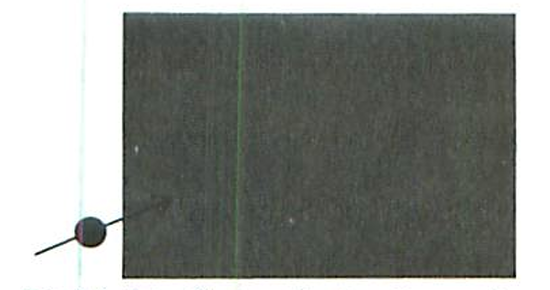
\includegraphics[width=.8\linewidth]{shot.png}
  \caption{The electron is shot into the gas}
  \label{fig:shot}
\end{subfigure}
\begin{subfigure}{.5\textwidth}
  \centering
  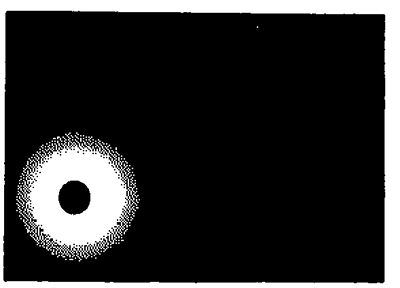
\includegraphics[width=.8\linewidth]{clothing.png}
  \caption{The electron creates holes as it moves along}
  \label{fig:clothing}
\end{subfigure}
\caption{Electron gas propagation taken from \textcite{mattuck_guide_1992}}
\label{fig:propagates}
\end{figure}
As it propagates through this medium, it will have an electrostatic repulsion with the electrons in the gas, so it will create holes (depicted in white) as it moves along (pictured in Figure \ref{fig:clothing}). Therefore, it no longer makes sense to think of the bare electron, but rather the quasi-electron along with its "clothing" of holes. To make this more rigorous, we have the equation
\begin{equation}
    \epsilon_{\text{quasi}} - \epsilon_{\text{bare}} = \epsilon_{\text{self}},
\end{equation}
which is saying that the difference between the quasi-electron energy and the bare electron energy can be thought of as the electron's self-energy, or just the energy of its "clothing". So we can think of $\epsilon_{\text{bare}}$ and $\epsilon_{\text{quasi}}$ as originating from the noninteracting and interacting Green's functions $G_0$ and $G$, respectively. The self-energy $\Sigma$ then captures the difference between these two quantities. Typically, $\Sigma $ is designed to capture all of the quantum mechanical effects of the many body system, including the exchange (partially captured by HF as noted in section \ref{sec:hf}) and correlation effects, so it is often denoted as $\Sigma_{xc}$.
\subsection{The $GW$ Approximation}
In order to solve the Dyson equation \ref{eqn:dyson}, we need to make approximations to the self-energy $\Sigma$. By introducing the screened Coulomb potential $W$, which represents the effective electrostatic interaction between electrons (as described above through the concept of the quasi-electron), the polarization function $P$, which describes the response of the system to the introduction of an electron, and the vertex function $\Gamma$, which describes the interaction between the electrons and holes, we can write down the five Hedin's equations
\begin{equation}
\begin{aligned}
& G(1,2)=G_0(1,2)+\int d(3,4) G_0(1,3) \Sigma(3,4) G(4,2) \\
& P(1,2)=\int d(3,4) G(1,3) G(4,1) \Gamma(3,4 ; 2) \\
& W(1,2)=V(1,2)+\int d(3,4) V(1,3) P(3,4) W(4,2) \\
& \Sigma(1,2)=\int d(3,4) G(1,3) \Gamma(3,2 ; 4) W(4,1) \\
& \Gamma(1,2 ; 3)=\delta(1,2) \delta(1,3)+\int d(4,5,6,7) \frac{\delta \Sigma(1,2)}{\delta G(4,5)} G(4,6) G(7,5) \Gamma(6,7 ; 3)
\end{aligned}
\end{equation}
where we have made use of the shorthand notation $1=(\mathbf{r}_1, t_1)$ and $V$ is the bare Coulomb potential. The $GW$ approximation is a simplification of these equations, where we neglect the vertex function $\Gamma$ by setting $\Gamma (1,2,3)= \delta (1,2) \delta (1,3)$. This simplifies the equations for the self-energy and polarization function to
\begin{equation}
\begin{aligned}
& \Sigma(1,2)=\int d(1,2) G(1,2) W(1,2) \\
& P(1,2)=\int d(1,2) G(1,2) G(2,1). \\
\end{aligned}
\end{equation}
\begin{figure}
    \centering
    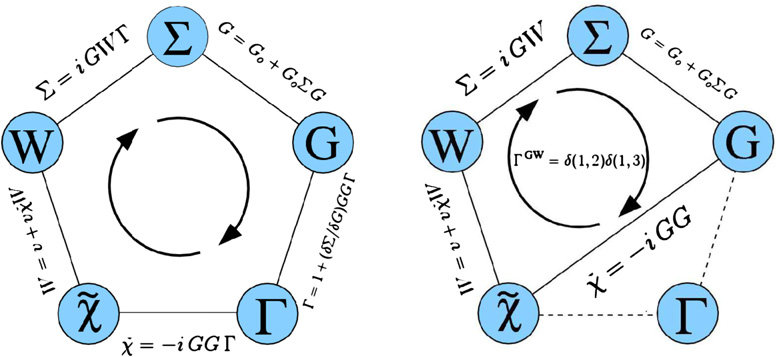
\includegraphics[width=\textwidth]{Left-panel-Graphical-representation-of-Hedins-equations-Right-panel-The-four-coupled.jpg}
    \caption{Graphical representation of Hedin's equations taken from \textcite{noauthor_frontiers_nodate}. The left panel shows the full set of equations, whereas the right panel shows the $GW$ approximation.}
    \label{fig:hedin}
\end{figure}
The figure \ref{fig:hedin} shows the self-consistency between these equations, with the polarization $P$ represented by $\tilde{\chi}$. Full self-consistency, including the vertex function $\Gamma$, is shown in the left panel, whereas the $GW$ approximation, which neglects the vertex function, is shown in the right panel. The $G_0W_0$ method, which I have studied, only performs one loop of the $GW$ approximation cycle. This is why it is often termed a "one-shot" procedure.
\subsection{Application in MBPT}
Now that we have the recipe to solve for its interacting version, the single-particle Green's function $G$ contains a lot of information that we would be interested in to provide an MBPT correction. In this work, we use it to update mean-field molecular orbital energies $\epsilon_{p}^0$ to quasiparticle energies $\epsilon_{p}^{QP}$, which are interpreted as effective molecular orbital energies. We also use it to update the electron density via the linearized $G_0W_0$ density matrix derived in chapter \ref{chap:linearized_gw}. Finally, we use it to determine the total energy of the molecule with different total energy functionals. It can also be used, among other things, to compute the spectral function, which gives access to ionization potentials and electron affinities. \autocite{noauthor_frontiers_nodate}






\chapter{$G_0W_0$ Procedure}
\section{Iterative equation}
The linearized procedure that was used in this work to compute quasiparticle energies, is given by
\begin{equation}
    \delta_{pq}F_{pq}^{HF}[\gamma^{MF}] + \Sigma _{c}(\varepsilon_{p}^{QP}) = \varepsilon_{p}^{QP}.
\label{eq: Iterative equation}
\end{equation}
The first term corresponds to taking the diagonal of the Hartree-Fock matrix $F_{pq}^{HF}$ evaluated at a given electron density $\gamma_{MF}$ These electron densities are obtained from a previous mean-field calculation, so $\gamma_{MF}$ means either $\gamma_{DFT}$ or $\gamma_{HF}$. The second term evaluates $\Sigma _{c}$ for the $\varepsilon_{p}^{QP}$ determined in the previous iteration. The right side of the equality gives the updated $\varepsilon_{p}^{QP}$.\\\\ Equation \ref{eq: Iterative equation} is iterated until self-consistency. We start with an initial guess for $\varepsilon_{p}^{QP}$, which is given by the mean-field orbital energy $\epsilon_p$. This is used in the first iteration to solve for the right-hand side $\varepsilon_{p}^{QP}$ of Equation \ref{eq: Iterative equation}. In the next iteration, we use the previously obtained $\varepsilon_{p}^{QP}$ to determine $\Sigma _{c}$. This process is repeated until we reach a convergence threshold for $\varepsilon_{p}^{QP}$. One can also use the Newton-Raphson method to solve the iterative equation for $\varepsilon_{p}^{QP}$.
\subsection{The Fock Matrix}
In section \ref{sec:hf}, we defined the Fock matrix. In the basis of molecular orbitals, it can be written by
\begin{equation}
    F_{ij}^{HF} = h_{ij} + \sum_{kl}^{occ} P_{kl} \left( (ij|kl) - \frac{1}{2} (ik|jl) \right),
\end{equation}
where $h_{ij}$ is the one-electron part of the Hamiltonian, $P_{kl}$ is the density matrix, and $(ij|kl)$ are the two-electron integrals.
\subsection{Correlation-Self Energy: Use}
$\Sigma _{c}$, tasked with capturing the electron correlation effects, is dynamic, as opposed to the previous Fock term that was discussed, as is updated with a new $\varepsilon_{p}^{QP}$ in each iteration. In the case of the $G_0W_0$ approximation, we use the common approximation, considering only the diagonal element of $\Sigma _{c}$ corresponding to the orbital with index $p$. This function is evaluated at the $\varepsilon_{p}^{QP}$ just obtained in the previous iteration. To summarize, we are actually interested in $\Sigma_{pp}^{corr}(\varepsilon_{p}^{QP})$. 
\subsection{Updated $\varepsilon_{p}^{QP}$}
This is the right side, or the solution, of Equation \ref{eq: Iterative equation}.



\section{Correlation Self-Energy}
\label{sec:correlation_self_energy}
\begin{equation}
    \Sigma_{pp}^{\text{corr}}(\omega) = \sum_{\mu }^{\text{RPA}}\left(\sum_{i}^{\text{occupied}} \frac{\textbf{V}_{pi}^{\mu }\textbf{V}_{ip}^{\mu }}{\omega -(\epsilon _{i}-\Omega  _{\mu })}+ \sum_{a}^{\text{virtual}} \frac{\textbf{V}_{pa}^{\mu }\textbf{V}_{ap}^{\mu }}{\omega -(\epsilon _{a}+\Omega  _{\mu })}\right)
\end{equation}
This is the working equation for the diagonal $pp$ of the correlation self-energy for a given MO. First, we have a sum running over all of the excitations obtained from the previous RPA calculation. Then, we have two terms: one sum running over all of the occupied orbitals and the other sum running over all virtual orbitals. The $\textbf{V}^{\mu}_{pq}$ and $\boldsymbol{\Omega ^{\mu}}$ are the residues and excitation energies, respectively, from the previous RPA calculation. $\omega$ is my input frequency and the $\epsilon_p$ are the orbital energies from my previous mean-field calculation.



\section{Random Phase Approximation}
The RPA is a linear response theory that is used to compute the excitation energies and vectors. The working matrix equation is given by \autocite{dreuw_single-reference_2005}
\begin{equation}
\begin{bmatrix}
\textbf{A} & \textbf{B} \\
-\textbf{B} & -\textbf{A}
\end{bmatrix}
\begin{bmatrix}
\textbf{X} \\
\textbf{Y}
\end{bmatrix}
= \boldsymbol{\Omega ^{(-\mu + \mu)}}
\begin{bmatrix}
\textbf{X} \\
\textbf{Y}
\end{bmatrix}
,
\label{eq: RPA matrix equation}
\end{equation}
where we define $\boldsymbol{\Omega} ^{(-\mu + \mu)}$ as a diagonal matrix containing the excitation and de-excitation energies, which have the same magnitude $\boldsymbol{\Omega}^{|\mu|}$. Accordingly, we just use the excitation energies in what follows which we simply denote as $\boldsymbol{\Omega ^{\mu}}$. The matrix
$\textbf{A}$ is defined as
\begin{equation}
    \textbf{A}_{ia,jb} = \delta _{ij}\delta _{ab}(\epsilon _{a}- \epsilon _{i}) + 2(ia||jb)
\label{eq: A matrix RPA}
\end{equation}
and $\textbf{B}$ is
\begin{equation}
    \textbf{B}_{ia,jb} = 2(ia||jb)
\label{eq: B matrix RPA}
\end{equation}
where the anti-symmetrized two-electron integrals are defined in Chapter \ref{chap:nomenclature}.

$\textbf{X}$ and $\textbf{Y}$ correspond to excitations and the de-excitations, respectively.
\subsection{Direct approximation}
Everywhere in this work, we consider the direct approximation, which just means that all instances of anti-symmetrized two-electron integrals are replaced by their direct counterparts, i.e., in Equation \ref{eq: A matrix RPA}, and Equation \ref{eq: B matrix RPA}, $(ia||jb) \rightarrow (ia|jb)$.

An alternative formulation that takes advantage of the symmetry obtained through neglect of the deexcitation energies and the direct formulation of the RPA (dRPA) can also be used and is derived in Appendix \ref{app:symm_drpa} as suggested by \textcite{furche_density_2001}.
\subsection{Residues}

The residue $\textbf{V}^{\mu}_{pq}$ is obtained by considering a contraction of two tensors. First, we consider the sum of the excitation vectors $\textbf{X}$ and $\textbf{Y}$ at the same excitation energy $\mu$: $\textbf{Z}_{i,a}^{\mu} = \textbf{X}_{i,a}^{\mu} + \textbf{Y}_{i,a}^{\mu}$. Then, we define the appropriate integrals for this excitation
\begin{equation}
    \textbf{W}_{p,q,i,a} = \sqrt{2} \sum_{p,q,i,a} (pq|ia).
\end{equation}
This factor of $\sqrt{2}$ comes from the spin integration of the restricted formalism that we use.
We define a combined occupied-virtual index $\nu$, so: $\textbf{Z}_{i,a}^{\mu} = \textbf{Z}_{\nu}^{\mu}$ and $\textbf{W}_{p,q,i,a} = \textbf{W}_{p,q,\nu}$.

And then we form the residue from
\begin{equation}
    \textbf{V}_{pq}^{\mu} = \sum_{\nu} \textbf{W}_{p,q,\nu} \textbf{Z}_{\nu}^{\mu}.
\end{equation}

\subsection{Tamm-Dancoff Approximation}
In this method, we neglect the $\textbf{B}$ matrix of the RPA equation. So the eigenvalue equation becomes
\begin{equation}
    \textbf{A}\textbf{X} = \boldsymbol{\Omega ^{\mu}} \textbf{X}
\end{equation}
where we still have:
\begin{equation}
    \textbf{A}_{ia,jb} = \delta _{ij}\delta _{ab}(\varepsilon _{a}- \varepsilon _{i}) + 2(ia||jb)
\label{eq: A matrix TDA}
\end{equation}
And then we follow the same procedure as in the RPA to get the residues $\textbf{V}_{pq}^{\mu}$, where now we have $\textbf{Z}_{\nu, \mu} = \textbf{X}_{\nu, \mu}$.

\chapter{Linearized $G_0W_0$ Density Matrix}
As noted earlier, we can get a density matrix out of the interacting Green's function. Then this allows us to obtain new MO coefficients through a rotation of those from the noninteracting Green's function. The form of this density matrix is shown below, and the derivation of it is given in Appendix \ref{app:linearized_gw}.
\label{chap:linearized_gw}
\subsection{Implementation}
These are the working equations in the spin-restricted formalism, which explains why we tack on the factor of 2. First, we consider the fully occupied block
\begin{equation}
\gamma_{ij}^{GW}=2\delta_{ij}-2\sum_{a\mu} \frac{\textbf{V}_{ia}^\mu \textbf{V}_{ja}^\mu}{\left(\epsilon_{i}-\epsilon_{a}-\boldsymbol{\Omega ^{\mu}}\right)\left(\epsilon_{j}-\epsilon_{a}-\boldsymbol{\Omega ^{\mu}}\right)},
\end{equation}
where the $\boldsymbol{\Omega ^{\mu}}$ are the excitation energies and the $\textbf{V}_{pq}^{\mu}$ are the transition vectors. The sum runs over all virtual orbitals and excitation energies. Next, we have the virtual-virtual block
\begin{equation}
\gamma_{ab}^{GW}=-2\sum_{i\mu} \frac{\textbf{V}_{ai}^{\mu} \textbf{V}_{bi}^{\mu}}{\left(\epsilon_{i}-\epsilon_{a}-\boldsymbol{\Omega ^{\mu}}\right)\left(\epsilon_{i}-\epsilon_{b}-\boldsymbol{\Omega ^{\mu}}\right)},
\end{equation}
where the sum runs over all occupied orbitals and excitation energies.
Finally, we have the mixed block
\begin{equation}
    \gamma_{i b}^{G W}=\frac{2}{\epsilon_{i}-\epsilon_{b}}\left[ \sum_{a \mu} \frac{\textbf{V}_{i a}^{\mu} \textbf{V}_{b a}^{\mu}}{\epsilon_{i}-\epsilon_{a}-\boldsymbol{\Omega ^{\mu}}} - \sum_{j \mu} \frac{\textbf{V}_{i j}^{\mu} \textbf{V}_{bj}^{\mu}}{\epsilon_{j}-\epsilon_{b}-\boldsymbol{\Omega ^{\mu}}} \right],
\end{equation}
where we have two sums; one over occupied orbitals and excitation energies and the other over virtual orbitals and excitation energies.
This all contributes to the form of the density matrix as:
\begin{equation}
    2\begin{pmatrix}
        \gamma _{i j}^{G W} & \gamma _{i b}^{G W} \\
        \gamma _{bi}^{G W } & \gamma _{a b}^{G W}
    \end{pmatrix}
\end{equation}
Where $\gamma _{bi}^{G W }$ is simply the transpose of $\gamma _{ib}^{\text{GW}}$, since all elements of this matrix are real. Therefore, this density matrix is Hermitian.



\chapter{Results}
\subsection{Graphical vs. Iterative}
Equation \ref{eq: Iterative equation} can be solved iteratively, but also graphically in the HF case by plotting $\Sigma _{c}$ as a function of the input frequency, which takes on  the possible values for $\varepsilon_{p}^{QP}$. Since $F_{pq}^{HF}$ is diagonal in the canonical HF MO basis, Equation \ref{eq: Iterative equation} can be reformulated as
\begin{equation}
    \epsilon _{p}^{HF} + \Sigma_{pp}^{corr}(\omega) = \omega  \rightarrow \Sigma_{pp}^{corr}(\omega) = \omega  - \epsilon _{p}^{HF}.
\end{equation}
As can be seen in figure \ref{fig:graphic}, the line at $\omega - \epsilon_{p}^{HF}$ intersects with $\Sigma _{c}$ at the same $\varepsilon_{p}^{QP}$ that we get from our iterative procedure, namely at the $\omega = -12.18 eV$.
 This is a useful check to see if the self-energy, which we defined in section \ref{sec:correlation_self_energy}, has been computed correctly.
\begin{figure}[h]
    \centering
    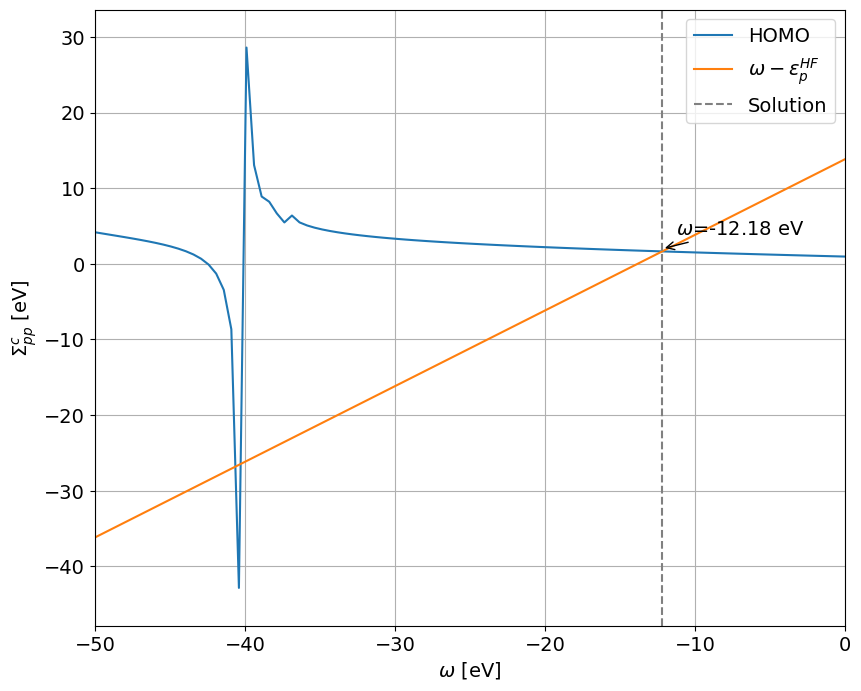
\includegraphics[width=\textwidth]{correlation_energies.png}
\caption{Graphical solution of the correlation self-energy for the HOMO of $H_2O$}
\label{fig:graphic}
\end{figure}
Also, at around $\omega$ = -40 eV, one can observe a pole structure. This would pose problems for the convergence of my iterative procedure Equation \ref{eq: Iterative equation} if the $\varepsilon_{p}^{QP}$ that I was looking for was close to this $\omega $ value. 
\subsection{Testing of equation \ref{eq: Iterative equation}}
Additional tests for a range of molecules and MOs with my implementation are reported in table \ref{tab:tests}.
\begin{table}[h]
\centering
\caption{Tests of my dRPA and dTDA implementations of $G_0W_0$. Energy deviations (in eV) for my implementation of the exact analytic $G_0W_0$ with dTDA and dRPA for different molecules across a range of orbitals versus that of PySCF.}
\label{tab:energies}
\resizebox{\textwidth}{!}{%
\begin{tabular}{|c|c|c|c|c|c|c|c|c|c|c|}
\hline
\multirow{2}{*}{Orbital} & \multicolumn{2}{c|}{$H_2O$} & \multicolumn{2}{c|}{$HCl$} & \multicolumn{2}{c|}{$NH_3$} & \multicolumn{2}{c|}{$LiH$} & \multicolumn{2}{c|}{$CO$} \\
\cline{2-11}
                         & dTDA & dRPA & dTDA & dRPA & dTDA & dRPA & dTDA & dRPA & dTDA & dRPA \\
\hline
HOMO - 2 & 1.78e-15 & 5.33e-15 & 1.42e-14 & 2.13e-12 & 5.33e-15 & 1.42e-14 & 4.21e-10 & 3.55e-14 & 1.73e-10 & 0.00477 \\
\hline
HOMO - 1 & 2.31e-14 & 1.07e-13 & 1.30e-12 & 5.24e-13& 3.55e-15 & 2.33e-10 & 4.55e-12 & 2.84e-14 & 1.73e-10 & 0.00476 \\
\hline
HOMO     & 4.44e-15 & 2.84e-13 & 1.48e-12 & 5.71e-13 & 1.67e-11 & 1.30e-12 & 1.33e-15 & 1.96e-10 & 1.06e-12 & 2.84e-13 \\
\hline
LUMO     & 3.43e-14 & 2.65e-14 & 4.44e-16 & 1.24e-12 & 8.60e-14 & 8.78e-14 & 1.11e-15 & 2.66e-15 & 2.22e-15 & 0.00679 \\
\hline
LUMO + 1 & 2.14e-13 & 2.71e-14 & 2.22e-13 & 1.04e-10 & 4.40e-13 & 8.78e-14 & 1.12e-12 & 2.43e-14 & 3.11e-15 & 0.00678 \\
\hline
LUMO + 2 & 4.07e-11 & 6.92e-10 & 7.11e-15 & 1.18e-10 & 3.15e-14 & 4.97e-14 & 1.12e-12 & 3.09e-14 & 3.99e-14 & 3.99e-14 \\
\hline
\end{tabular}
}
\label{tab:tests}
\end{table}

The cc-pVDZ basis set was used for all calculations. As can be seen, my deviations from PySCF are near floating point error with the exception of my dRPA calculation for $CO$.
\subsection{Total energy functionals}

\begin{equation}
    E_{\text{tot}}^{GM} = T_s [\gamma  ] + V_H [\gamma  ] + V_x [\gamma  ] + V_{\text{nuc, elec}} [\gamma  ] + V_{\text{nuc, nuc}} + E_{\text{corr}} ^{\text{GM}}[\gamma_0 ]
\label{eq:GM}
\end{equation}

\begin{table}[h!]
    \centering
    \begin{tabular}{lcccc}
        \toprule
        & \textbf{MOLGW} & \textbf{FHI-AIMS} & \textbf{Mine from eqn. \ref{eq:GM}} & \textbf{Deviation} \\
        \midrule
        \textbf{He} & -0.759780 & -0.759737 & -0.759781 & -0.000043 \\
        \textbf{Ne} & -0.120554 & -0.120551 & -0.120553 & -0.000002 \\
        \bottomrule
    \end{tabular}
    \caption{Galitskii-Migdal correlation energies (in Hartrees) using HF as the mean field object. Deviations are calculated with the difference between my implementation and the average of those from MOLGW and FHI-AIMS.}
\end{table}


\begin{table}[h!]
    \centering
    \begin{tabular}{lccc}
        \toprule
        & \textbf{PySCF} & \textbf{Mine from eqn. \ref{eq:klein1}} & \textbf{Mine from eqn. \ref{eq:klein2}} \\
        \midrule
        \textbf{H$_2$O} & -76.2059 & -76.0673 & -75.9822 \\
        \textbf{NH$_3$} & -56.3946 & -56.2540 & -56.1794 \\
        \textbf{LiH} & -8.02132 & -8.04017 & -7.98422 \\
        \bottomrule
    \end{tabular}
    \caption{Comparison of Klein total energies (in Hartrees) between PySCF and my implementation.}
\end{table}
\begin{equation}
    E_{\text{tot}} = T_s [\gamma _{0}] + V_H [\gamma ] + V_x [\gamma ] + V_{\text{nuc, elec}} [\gamma ] + V_{\text{nuc, nuc}} + E_{\text{corr}} ^{\text{Klein}}[\gamma ]
\label{eq:klein1}
\end{equation}
\begin{equation}
    E_{\text{tot}} = T_s [\gamma ] + V_H [\gamma ] + V_x [\gamma ] + V_{\text{nuc, elec}} [\gamma ] + V_{\text{nuc, nuc}} + E_{\text{corr}} ^{\text{Klein}}[\gamma_0]
\label{eq:klein2}
\end{equation}

\begin{table}[h!]
    \centering
    \begin{tabular}{lccc}
        \toprule
        & \textbf{Mine from eqn. \ref{eq:klein1}} & \textbf{Mine from eqn. \ref{eq:klein2}} & \textbf{Difference} \\
        \midrule
        \textbf{H$_2$O} & -0.317604 & -0.232507 & -0.085097 \\
        \textbf{NH$_3$} & -0.297227 & -0.222575 & -0.074652 \\
        \textbf{LiH} & -0.093758 & -0.037806 & -0.055952 \\
        \bottomrule
    \end{tabular}
    \caption{Difference in correlation energies (in Hartrees) between my two implementations of the Klein functional.}
\end{table}


\subsection{Plotting natural occupations}
The natural occupations are found by diagonalizing the density matrix. They are interpreted as being the number of electrons in a given orbital.\autocite{szabo_modern_2012} Here we considered the one-electron density matrix from multiple methods: restricted Hartree-Fock, which contains no correlation for the single particles, and Full Configuration Interaction (FCI), which contains the exact correlation. As can be seen in Figure \ref{fig:h2_dissociation}, our implementation of the Linearized $G_0W_0$ Density Matrix in the direct Random Phase Approximation (dRPA) and direct Tamm-Dancoff Approximation (dTDA) gives a portion of this correlation.
\begin{figure}[h]
    \centering
    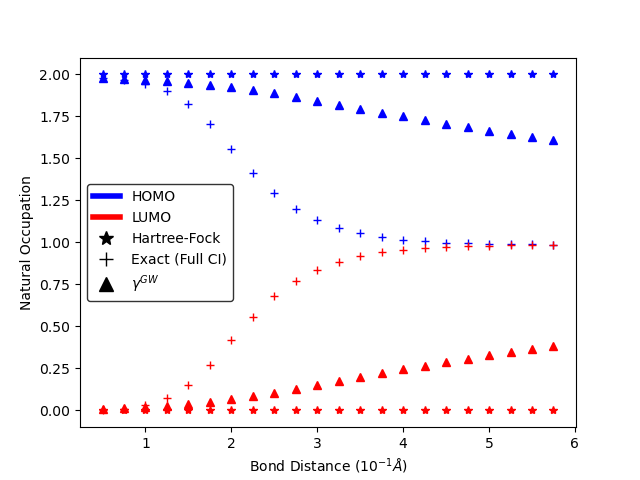
\includegraphics[width=\textwidth]{h2_occupations.png}
\caption{Natural occupations of the HOMO (State 1) and LUMO (State 2) of $H_2$ along the dissociation coordinate}
\label{fig:h2_dissociation}
\end{figure}
When $H_2$ is at the though bond distance near equate bum, we see in Figure \ref{fig:h2_dissociation} that the HOMO is fully occupied with 2 electrons, while the LUMO is unoccupied. This situation is represented by the simple MO diagram in Figure \ref{fig:h2_mo_diagram}. As the molecule dissociates, the orbital occupations for the restricted Hartree-Fock method do not change at all, while FCI, containing the exact correlation, gives the expected result of the HOMO and LUMO both having occupations of 1 electron. The dRPA and dTDA fall somewhere in between these two extremes.
\begin{figure}[h]
    \centering
    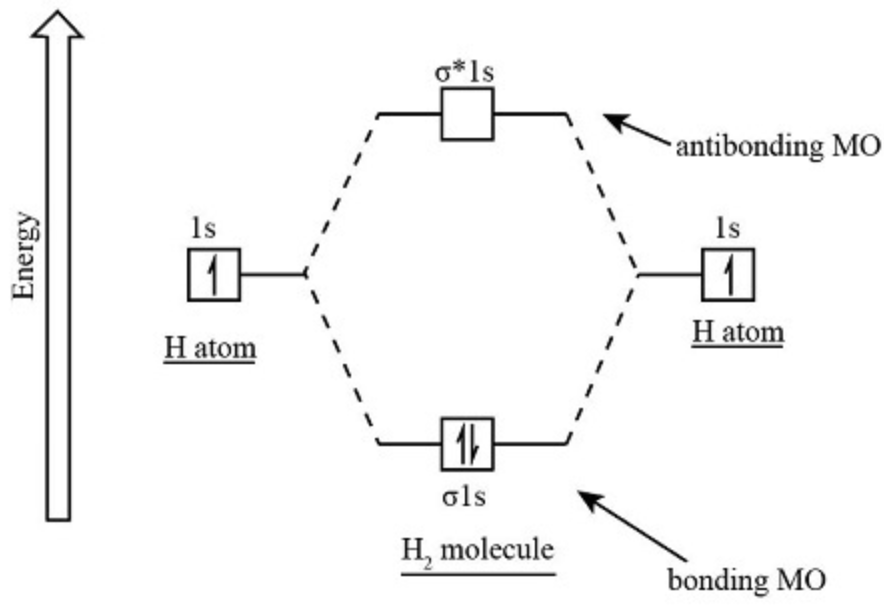
\includegraphics[width=\textwidth]{h2_mo.png}
\caption{MO diagram of $H_2$ at the equilibrium bond distance. Notice that the HOMO is fully occupied with 2 electrons, while the LUMO is unoccupied. Diagram taken from the web \autocite{noauthor_molecular_nodate}}
\label{fig:h2_mo_diagram}
\end{figure}

\printbibliography[heading=bibintoc]

\appendix

\chapter{Symmetric formulation of the dRPA}
\label{app:symm_drpa}
Since we know that the excitation and de-excitation energies for the RPA are the same in magnitude, we can simplify the matrix equation to:
\begin{equation}
\begin{bmatrix}
\textbf{A} & \textbf{B} \\
-\textbf{B} & -\textbf{A}
\end{bmatrix}
\begin{bmatrix}
\textbf{X} \\
\textbf{Y}
\end{bmatrix}
= \boldsymbol{\Omega^{|\mu|} }
\begin{bmatrix}
\textbf{X} \\
\textbf{Y}
\end{bmatrix}
.
\end{equation}
In what follows, we will take $\boldsymbol{\Omega }$ to mean $\boldsymbol{\Omega^{|\mu|} }$.
The linearity suggests breaking down the problem into a set of linear equations
\begin{align}
    \textbf{AX} + \textbf{BY} &= \boldsymbol{\Omega } \textbf{X}\\
    -\textbf{BX}-\textbf{AY} &= \boldsymbol{\Omega } \textbf{Y},
\label{eqn:linearity}
\end{align}
which can be simplified by the addition of these two equations in \ref{eqn:linearity}
\begin{equation}
    (\textbf{A}-\textbf{B})(\textbf{X}-\textbf{Y})= \boldsymbol{\Omega } (\textbf{X}+\textbf{Y})
\label{eqn:for_addition}
\end{equation}
which can be rearranged to give
\begin{equation}
    (\textbf{X}+\textbf{Y}) = \boldsymbol{\Omega }^{-1}(\textbf{A}-\textbf{B})(\textbf{X}-\textbf{Y}).
\label{eqn:addition}
\end{equation}
Doing a pairwise subtraction of the equations in \ref{eqn:linearity} instead gives
\begin{equation}
    (\textbf{A}+\textbf{B})(\textbf{X}+\textbf{Y})= \boldsymbol{\Omega } (\textbf{X}-\textbf{Y}). 
\label{eqn:for_subtraction}
\end{equation}
Similarly, we can isolate
\begin{equation}
    (\textbf{X}-\textbf{Y}) = \boldsymbol{\Omega }^{-1}(\textbf{A}+\textbf{B})(\textbf{X}+\textbf{Y}).
\label{eqn:subtraction}
\end{equation}
Equations \ref{eqn:for_addition} and \ref{eqn:for_subtraction} can be combined to get
\begin{equation}
    \boldsymbol{\Omega } = (\textbf{X}-\textbf{Y})^{\dag} (\textbf{A}-\textbf{B})(\textbf{X}-\textbf{Y})
\end{equation}
and
\begin{equation}
    \boldsymbol{\Omega } = (\textbf{X}+\textbf{Y})^{\dag} (\textbf{A}+\textbf{B})(\textbf{X}+\textbf{Y}).
\end{equation}
Substituting in for $\textbf{X}+\textbf{Y}$ from \ref{eqn:addition} into equation \ref{eqn:for_subtraction}
\begin{equation}
    \boldsymbol{\Omega }^{-1}(\textbf{A}+\textbf{B})(\textbf{A}-\textbf{B})(\textbf{X}-\textbf{Y}) = \boldsymbol{\Omega } (\textbf{X}-\textbf{Y}).
\end{equation}
Multiplication by $\boldsymbol{\Omega }$ gives
\begin{equation}
    (\textbf{A}+\textbf{B})(\textbf{A}-\textbf{B})(\textbf{X}-\textbf{Y}) = \boldsymbol{\Omega }^2 (\textbf{X}-\textbf{Y}).
\end{equation}
Now, we plug the definition in equation \ref{eqn:subtraction} for the $(\textbf{X}-\textbf{Y})$ terms
\begin{equation}
    (\textbf{A}+\textbf{B})(\textbf{A}-\textbf{B})\boldsymbol{\Omega }^{-1}(\textbf{A}+\textbf{B})(\textbf{X}+\textbf{Y}) = \boldsymbol{\Omega }^2 \boldsymbol{\Omega }^{-1}(\textbf{A}+\textbf{B})(\textbf{X}+\textbf{Y}).
\end{equation}
Multiplication through by $\boldsymbol{\Omega }$ gives and $(\textbf{A}+\textbf{B})^{-1}$ gives
\begin{equation}
    (\textbf{A}-\textbf{B})(\textbf{A}+\textbf{B})(\textbf{X}+\textbf{Y}) = \boldsymbol{\Omega }^{2} (\textbf{X}+\textbf{Y}).
\end{equation}
At this point we want to define $\textbf{T}=(\textbf{A}-\textbf{B})^{-\frac{1}{2}}(\textbf{X}+\textbf{Y})$, so that we can write
\begin{equation}
    (\textbf{A}-\textbf{B})(\textbf{A}+\textbf{B})(\textbf{A}-\textbf{B})^{\frac{1}{2}}\textbf{T} = \boldsymbol{\Omega }^{2} (\textbf{A}-\textbf{B})^{\frac{1}{2}}\textbf{T}.
\end{equation}
Dividing through by $(\textbf{A}-\textbf{B})^{\frac{1}{2}}$ gives:
\begin{equation}
    (\textbf{A}-\textbf{B})^{\frac{1}{2}}(\textbf{A}+\textbf{B})(\textbf{A}-\textbf{B})^{\frac{1}{2}}\textbf{T} = \boldsymbol{\Omega }^{2} \textbf{T}.
\label{eqn:final}
\end{equation}
We can solve this matrix equation now. We can use this definition for $\textbf{T}$ to redefine equation \ref{eqn:addition} 
\begin{equation}
    (\textbf{X}+\textbf{Y}) = (\textbf{A}-\textbf{B})^{\frac{1}{2}}\textbf{T}.
\end{equation}
And then for normalization, we need
\begin{equation}
    (\textbf{X}-\textbf{Y})^{\dag}(\textbf{X}+\textbf{Y})=1.
\end{equation}
So we need
\begin{equation}
    (\textbf{X}-\textbf{Y})=(\textbf{A}-\textbf{B})^{-1}(\textbf{X}+\textbf{Y})\boldsymbol{\Omega } .
\end{equation}
So we can instead use the solution of equation \ref{eqn:final} to obtain the excitation energies $\boldsymbol{\Omega }^{\mu}$ and the excitation vectors $\textbf{X}^{\mu}$ and $\textbf{Y}^{\mu}$, the latter of which we will then use to construct our residues $\textbf{V}^{\mu}_{pq}$.














\chapter{Derivation of the linearized $G_0W_0$ density matrix}
This derivation will be carried out in the spin-unrestricted formalism.
\label{applinearized_gw}
We have the equation for the density matrix
\begin{equation}
\begin{aligned}
\gamma^\sigma\left(\mathbf{r}_1, \mathbf{r}_2\right)= & \gamma_0^\sigma\left(\mathbf{r}_1, \mathbf{r}_2\right) -\frac{\mathrm{i}}{2 \pi} \int \mathrm{d} \mathbf{r}_3 \mathrm{~d} \mathbf{r}_4 \mathrm{~d} \omega \mathrm{e}^{\mathrm{i \omega \eta}} G_0^\sigma\left(\mathbf{r}_1, \mathbf{r}_3, \omega\right) \Sigma_c^\sigma\left(\mathbf{r}_3, \mathbf{r}_4, \omega\right) G_0^\sigma\left(\mathbf{r}_4, \mathbf{r}_2, \omega\right)
\label{eqninit_dm}
\end{aligned}
\end{equation}
where $\gamma^\sigma$ is our new density matrix from the interacting Green's function, and $\gamma_0^\sigma$ is the density matrix from the noninteracting Green's function. $\omega$ is the frequency and $\eta$ is a small infinitesimal positive number, which we will later take to be zero. $G_0^\sigma(\omega)$ and $\Sigma_c^\sigma(\omega)$ are the noninteracting Green's function and the correlation self-energy, respectively, now Fourier transformed to the frequency domain.
In order to simplify the integral, let us consider
\begin{equation}
I = \int \mathrm{d} \mathbf{r}_3 \mathrm{~d} \mathbf{r}_4  G_0^\sigma\left(\mathbf{r}_1, \mathbf{r}_3\right) \Sigma_c^\sigma\left(\mathbf{r}_3, \mathbf{r}_4\right) G_0^\sigma\left(\mathbf{r}_4, \mathbf{r}_2\right)
\end{equation}
The noninteracting Green's function in the MO basis is defined as
\begin{equation}
G_0\left(\mathbf{r}_1, \mathbf{r}_2, \right) = \sum_{pq} \phi_p^*(\mathbf{r}_1) G_{p q} \phi_q(\mathbf{r}_2)
\end{equation}
and likewise for the self-energy
\begin{equation}
\Sigma_c\left(\mathbf{r}_1, \mathbf{r}_2, \right) = \sum_{pq} \phi_p^*(\mathbf{r}_1) \Sigma_{c pq} \phi_q(\mathbf{r}_2)
\end{equation}
where $G_{p q}$ and $\Sigma_{p q}$ are the matrix elements of the noninteracting Green's function and the self-energy, respectively. We can rewrite the integral as
\begin{equation}
I_1 = \sum_{pq} \sum_{rs} \sum_{tu} \int \mathrm{d} \mathbf{r}_3 \mathrm{~d} \mathbf{r}_4 \phi_p^*(\mathbf{r}_1) G_{p q} \phi_q(\mathbf{r}_3) \phi_r^*(\mathbf{r}_3) \Sigma_{r s} \phi_s(\mathbf{r}_4) \phi_t^*(\mathbf{r}_4) G_{t u} \phi_u(\mathbf{r}_2)
\end{equation}
We can get rid of the integral over spatial indices by using the orthonormality of the basis functions.
\begin{equation}
I_1 = \sum_{pq} \sum_{r} \sum_{t} \phi_p^*(\mathbf{r}_1) G_{p r} \phi_r(\mathbf{r}) \phi_r^*(\mathbf{r}) \Sigma_{r t} \phi_t(\mathbf{r}^\prime) \phi_t^*(\mathbf{r}^\prime) G_{t q} \phi_q(\mathbf{r}_2)
\end{equation}
We use this and then also rewrite equation \ref{eqninit_dm} in terms of elements of the density matrix with
\begin{equation}
D_{p q \sigma}=\left\langle p \sigma\left|\gamma^\sigma\right| q \sigma\right\rangle
\end{equation}
to get
\begin{equation}
    D_{p q \sigma}=\bra{p\sigma } \gamma _0^\sigma \ket{q\sigma } -\frac{\mathrm{i }}{2 \pi} \sum_{r} \sum_{t} \int_{-\infty }^{\infty } \mathrm{d} \omega \mathrm{e}^{\mathrm{i \omega \eta}} \bra{p\sigma } G_0^\sigma (\omega) \ket{r\sigma } \bra{r\sigma } \Sigma_c^\sigma (\omega) \ket{t\sigma } \bra{t\sigma } G_0^\sigma (\omega) \ket{q\sigma }.
\label{eqnmo_dm}
\end{equation}
Next, we plug in the following definitions for the two different time orderings for the noninteracting Green's function and correlation piece of the self energy
\begin{equation}
G_{0 pq}^\sigma=\sum_i \frac{\delta_{pq} \delta_{pi}}{\omega-\epsilon_{i\sigma}-\mathrm{i}\eta}+\sum_a \frac{\delta_{pq} \delta_{pa}}{\omega-\epsilon_{a\sigma}+\mathrm{i}\eta}
\end{equation}
and
\begin{equation}
\begin{aligned}
\Sigma_{c p q}^\sigma(\omega)= & \sum_{i s} \frac{w_{p i \sigma}^s w_{q i \sigma}^s}{\omega-\epsilon_{i \sigma}+\Omega_s-\mathrm{i} \eta} +\sum_{a s} \frac{w_{p a \sigma}^s w_{q a \sigma}^s}{\omega-\epsilon_{a \sigma}-\Omega_s+\mathrm{i} \eta}
\end{aligned}
\end{equation}
into equation \ref{eqnmo_dm} to get
\begin{equation}
\begin{aligned}
D_{p q \sigma}= & \bra{p\sigma } \gamma _0^\sigma \ket{q\sigma } -\frac{\mathrm{i }}{2 \pi} \sum_{r} \sum_{t} \int_{-\infty }^{\infty } \mathrm{d} \omega \mathrm{e}^{\mathrm{i \omega \eta}} \left( \sum_i \frac{\delta_{p r} \delta_{p i}}{\omega-\epsilon_{i \sigma}-\mathrm{i} \eta}+\sum_a \frac{\delta_{p r} \delta_{p a}}{\omega-\epsilon_{a \sigma}+\mathrm{i} \eta} \right)\\
& \left( \sum_{k s} \frac{w_{r k \sigma}^s w_{t k \sigma}^s}{\omega-\epsilon_{k \sigma}+\Omega_s-\mathrm{i} \eta} +\sum_{c s} \frac{w_{r c \sigma}^s w_{t c \sigma}^s}{\omega-\epsilon_{c \sigma}-\Omega_s+\mathrm{i} \eta} \right) \left( \sum_j \frac{\delta_{t q} \delta_{t j}}{\omega-\epsilon_{j \sigma}-\mathrm{i} \eta}+\sum_b \frac{\delta_{t q} \delta_{t b}}{\omega-\epsilon_{b \sigma}+\mathrm{i} \eta} \right).
\end{aligned}
\end{equation}
Let us distribute the integral, which spawns 8 terms. Also note that the delta functions will get rid of the sums over r and t
\begin{equation}
\begin{aligned}
I_2 = \int_{-\infty }^{\infty }\mathrm{d} \omega \mathrm{e}^{\mathrm{i \omega \eta}} 
& \left( \sum_{ijks} \left( \frac{w_{i k \sigma}^s w_{j k \sigma}^s}{(\omega-\epsilon_{k \sigma}+\Omega_s-\mathrm{i} \eta)(\omega-\epsilon_{i \sigma}-\mathrm{i} \eta)(\omega-\epsilon_{j \sigma}-\mathrm{i} \eta)} \right) \right.\\
& \left. + \sum_{ibks} \left( \frac{w_{i k \sigma}^s w_{b k \sigma}^s}{(\omega-\epsilon_{k \sigma}+\Omega_s-\mathrm{i} \eta)(\omega-\epsilon_{i \sigma}-\mathrm{i} \eta)(\omega-\epsilon_{b \sigma}+\mathrm{i} \eta)} \right) \right.\\
& \left. + \sum_{ijcs} \left( \frac{w_{i c \sigma}^s w_{j c \sigma}^s}{(\omega-\epsilon_{c \sigma}-\Omega_s+\mathrm{i} \eta)(\omega-\epsilon_{i \sigma}-\mathrm{i} \eta)(\omega-\epsilon_{j \sigma}-\mathrm{i} \eta)} \right) \right.\\
& \left. + \sum_{ibcs} \left( \frac{w_{i c \sigma}^s w_{b c \sigma}^s}{(\omega-\epsilon_{c \sigma}-\Omega_s+\mathrm{i} \eta)(\omega-\epsilon_{i \sigma}-\mathrm{i} \eta)(\omega-\epsilon_{b \sigma}+\mathrm{i} \eta)} \right) \right. \\
& \left. + \sum_{ajks} \left( \frac{w_{a k \sigma}^s w_{j k \sigma}^s}{(\omega-\epsilon_{k \sigma}+\Omega_s-\mathrm{i} \eta)(\omega-\epsilon_{a \sigma}+\mathrm{i} \eta)(\omega-\epsilon_{j \sigma}-\mathrm{i} \eta)} \right) \right.\\
& \left. + \sum_{abks} \left( \frac{w_{a k \sigma}^s w_{b k \sigma}^s}{(\omega-\epsilon_{k \sigma}+\Omega_s-\mathrm{i} \eta)(\omega-\epsilon_{a \sigma}+\mathrm{i} \eta)(\omega-\epsilon_{b \sigma}+\mathrm{i} \eta)} \right) \right.\\
& \left. + \sum_{ajcs} \left( \frac{w_{a c \sigma}^s w_{j c \sigma}^s}{(\omega-\epsilon_{c \sigma}-\Omega_s+\mathrm{i} \eta)(\omega-\epsilon_{a \sigma}+\mathrm{i} \eta)(\omega-\epsilon_{j \sigma}-\mathrm{i} \eta)} \right) \right.\\
& \left. + \sum_{abcs} \left( \frac{w_{a c \sigma}^s w_{b c \sigma}^s}{(\omega-\epsilon_{c \sigma}-\Omega_s+\mathrm{i} \eta)(\omega-\epsilon_{a \sigma}+\mathrm{i} \eta)(\omega-\epsilon_{b \sigma}+\mathrm{i} \eta)} \right) \right)
\label{eqnexpanded_integral}
\end{aligned}
\end{equation}
At this point, we note the following relation between integrals $\oint_{D_{\pm}} f(z) = \int_{-R}^R f(z) + \int_{{C_R}_{\pm}} f(z)$. $D_{\pm}$ is a semicircular domain in either half of the complex plane, ${C_R}_{\pm}$ is the semicircle in the upper or lower part of the complex plane, and $R$ is the radius of the semicircle. We are able to take $R\rightarrow \infty$ and since $f(z)=e^{i\omega \eta}g(z)$, where $g(z)$ is analytic on $D$ except for a finite number of poles, the integral over the semicircle will vanish by Jordan's lemma, leaving us with $\int_{-R=-\infty}^{R=\infty} f(z)= \oint_{D_{\pm}} f(z)$. 

\begin{figure}
    \centering
    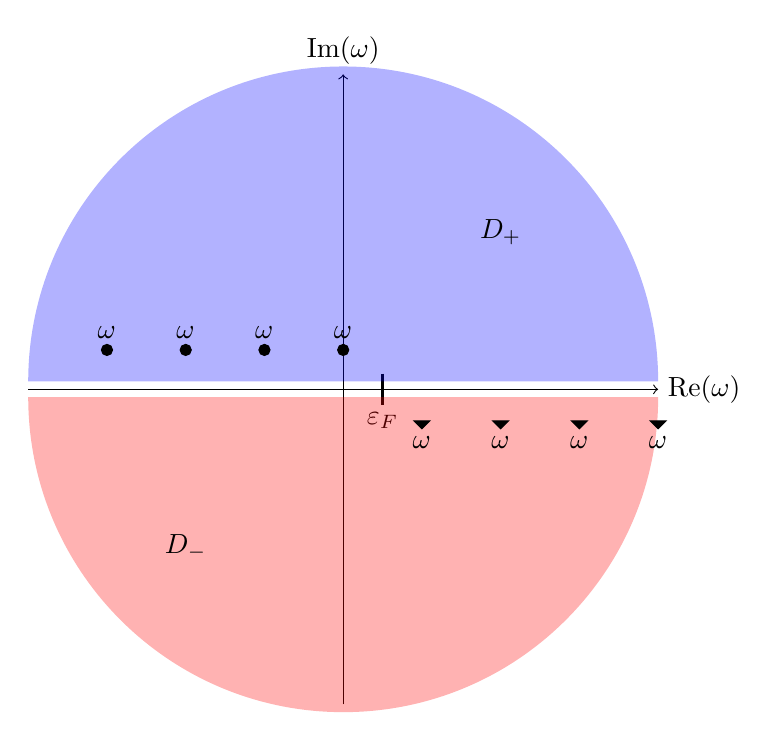
\begin{tikzpicture}
    % Draw the axes
    \draw[->] (-4, 0) -- (4, 0) node[right] {Re($\omega$)};
    \draw[->] (0, -4) -- (0, 4) node[above] {Im($\omega$)};
    
    % Draw the positive real axis label and tick mark for \varepsilon_{F}
    \draw[thick] (0.5, 0.2) -- (0.5, -0.2);
    \node at (0.5, -0.4) {$\varepsilon_{F}$};


    % Draw the semicircle contours
    % fill in its under side
    \fill[blue, opacity=0.3] (4, 0.1) arc[start angle=0, end angle=180, radius=4];
    \fill[red, opacity=0.3] (4, -0.1) arc[start angle=0, end angle=-180, radius=4];
    
    % Draw the poles above the real axis
    \foreach \x in {-3,-2,-1,0} {
        \draw[fill=black] (\x, 0.5) circle (2pt);
    }
    \node at (-3, 0.7) {$\omega_{}$};
    \node at (-2, 0.7) {$\omega_{}$};
    \node at (-1, 0.7) {$\omega_{}$};
    \node at (0, 0.7) {$\omega_{}$};    

    % Draw the poles below the real axis
    \foreach \x in {1,2,3,4} {
        \draw[fill=black] (\x, -0.5) -- ++(0.1, 0.1) -- ++(-0.2, 0) -- cycle;
    }
    \node at (1, -0.7) {$\omega_{}$};
    \node at (2, -0.7) {$\omega_{}$};
    \node at (3, -0.7) {$\omega_{}$};
    \node at (4, -0.7) {$\omega_{}$};

    
    % Label the contours
    \node at (2, 2) {$D_+$};
    \node at (-2, -2) {$D_-$};
\end{tikzpicture}
\caption{Contour for the complex frequency integral. The poles are denoted by the various $\omega$. The Fermi energy is denoted by $\varepsilon_F$. The integration contour $D_+$ is the semicircle in the upper complex plane, while $D_-$ is the semicircle in the lower complex plane.}
\end{figure}


\section{Fully occupied block}
The contribution over the fully occupied block of the density matrix will be given by the following two terms in equation \ref{eqnexpanded_integral}
\begin{equation}
\begin{aligned}
I_{ij} =& \sum_{ks} w_{i k \sigma}^s w_{j k \sigma}^s \oint_{D+} \mathrm{d} \omega \mathrm{e}^{\mathrm{i \omega \eta}} \frac{1}{(\omega-\epsilon_{k \sigma}+\Omega_s-\mathrm{i} \eta)(\omega-\epsilon_{i \sigma}-\mathrm{i} \eta)(\omega-\epsilon_{j \sigma}-\mathrm{i} \eta)}\\
& + \sum_{cs} w_{i c \sigma}^s w_{j c \sigma}^s \oint_{D+} \mathrm{d} \omega \mathrm{e}^{\mathrm{i \omega \eta}} \frac{1}{(\omega-\epsilon_{c \sigma}-\Omega_s+\mathrm{i} \eta)(\omega-\epsilon_{i \sigma}-\mathrm{i} \eta)(\omega-\epsilon_{j \sigma}-\mathrm{i} \eta)}
\end{aligned}
.
\end{equation}
Due to the contour $D_+$ chosen for this case, we have poles for the first term at $\omega_{11} = \epsilon _{k\sigma } - \Omega _s + \mathrm{i} \eta$, $\omega_{12} = \epsilon _{i\sigma } + \mathrm{i} \eta$, and $\omega_{13} = \epsilon _{j\sigma } + \mathrm{i} \eta$. For such simple poles, the Cauchy residue theorem simplifies to
\begin{equation}
\operatorname{Res}_{\omega =\omega _0} f(\omega )= \phi^{}\left(\omega _0\right)
\label{eqncauchy_residue}
\end{equation}
where $\phi_{\omega _0}(\omega ) = (\omega - \omega_0) f(\omega )$. For the first of these integrals in the occupied block, we have
\begin{equation}
f_1(\omega) = \frac{e^{i\omega \eta }}{(\omega-\epsilon_{k \sigma}+\Omega_s-\mathrm{i} \eta)(\omega-\epsilon_{i \sigma}-\mathrm{i} \eta)(\omega-\epsilon_{j \sigma}-\mathrm{i} \eta)}.
\end{equation}
% Plugging in $\omega_{11} = \epsilon _{k\sigma } - \Omega _s + \mathrm{i} \eta$, we get
% \begin{equation}
% \phi_{\omega_{11}}(\omega) = (\omega - \epsilon_{k \sigma} + \Omega_s - \mathrm{i} \eta) f_1(\omega) = \frac{e^{i\omega \eta }}{(\omega-\epsilon_{i \sigma}-\mathrm{i} \eta)(\omega-\epsilon_{j \sigma}-\mathrm{i} \eta)}
% \end{equation}
So at the first pole, in the limit $\eta \to 0$, we get
\begin{equation}
\phi_{\omega_{11}}(\epsilon_{k \sigma} - \Omega_s + \mathrm{i} \eta) = \frac{1}{(\epsilon_{k \sigma} - \Omega_s -\epsilon_{i \sigma})(\epsilon_{k \sigma} - \Omega_s -\epsilon_{j \sigma})}
\end{equation}
For the other poles, the procedure is similar with
\begin{equation}
\phi_{\omega_{12}}(\epsilon_{i \sigma} + \mathrm{i} \eta) = \frac{1}{(\epsilon_{i \sigma} -\epsilon_{k \sigma}+\Omega_s)(\epsilon_{i \sigma} -\epsilon_{j \sigma})}
\end{equation}
and
\begin{equation}
\phi_{\omega_{13}}(\epsilon_{j \sigma} + \mathrm{i} \eta) = \frac{1}{(\epsilon_{j \sigma} -\epsilon_{k \sigma}+\Omega_s)(\epsilon_{j \sigma} -\epsilon_{i \sigma})}.
\end{equation}
We move on to the second integral in the occupied block. It only has two poles in the fully occupied contour $\omega_{21} = \epsilon _{i\sigma } + \mathrm{i} \eta$ and $\omega_{22} = \epsilon _{j\sigma } + \mathrm{i} \eta$. We have $f_2(\omega)$ as
\begin{equation}
f_2(\omega) = \frac{e^{i\omega \eta }}{(\omega-\epsilon_{c \sigma}-\Omega_s+\mathrm{i} \eta)(\omega-\epsilon_{i \sigma}-\mathrm{i} \eta)(\omega-\epsilon_{j \sigma}-\mathrm{i} \eta)}.
\end{equation}
So $\phi_{\omega_{21}}(\omega _{21})$ is
\begin{equation}
\phi_{\omega_{21}}(\epsilon_{i \sigma} + \mathrm{i} \eta) = \frac{1}{(\epsilon_{i \sigma} -\epsilon_{c \sigma}-\Omega_s)(\epsilon_{i \sigma} -\epsilon_{j \sigma})}.
\end{equation}
Now we consider the second pole at $\omega_{22} = \epsilon _{j\sigma } + \mathrm{i} \eta$
\begin{equation}
\phi_{\omega_{22}}(\epsilon_{j \sigma} + \mathrm{i} \eta) = \frac{1}{(\epsilon_{j \sigma} -\epsilon_{c \sigma}-\Omega_s)(\epsilon_{j \sigma} -\epsilon_{i \sigma})}.
\end{equation}
We summarize the results in a table \ref{tabpoles_residues_occupied}.\\
\begin{table}[h]
\centering
\caption{Summary of Poles and their Residues}
\begin{tabular}{|c|c|c|}
\hline
Pole Notation & Position $\omega_0$ & Residue $\phi_{\omega_0}(\omega_0)$ \\
\hline
\multicolumn{3}{|c|}{Series $\omega_1$} \\
\hline
$\omega_{11}$ & $\epsilon_{k \sigma} - \Omega_s + \mathrm{i} \eta$ & $\frac{1}{(\epsilon_{k \sigma} - \Omega_s -\epsilon_{i \sigma})(\epsilon_{k \sigma} - \Omega_s -\epsilon_{j \sigma})}$ \\
$\omega_{12}$ & $\epsilon_{i \sigma} + \mathrm{i} \eta$ & $\frac{1}{(\epsilon_{i \sigma} -\epsilon_{k \sigma}+\Omega_s)(\epsilon_{i \sigma} -\epsilon_{j \sigma})}$ \\
$\omega_{13}$ & $\epsilon_{j \sigma} + \mathrm{i} \eta$ & $\frac{1}{(\epsilon_{j \sigma} -\epsilon_{k \sigma}+\Omega_s)(\epsilon_{j \sigma} -\epsilon_{i \sigma})}$ \\
\hline
\multicolumn{3}{|c|}{Series $\omega_2$} \\
\hline
$\omega_{21}$ & $\epsilon_{i \sigma} + \mathrm{i} \eta$ & $\frac{1}{(\epsilon_{i \sigma} -\epsilon_{c \sigma}-\Omega_s)(\epsilon_{i \sigma} -\epsilon_{j \sigma})}$ \\
$\omega_{22}$ & $\epsilon_{j \sigma} + \mathrm{i} \eta$ & $\frac{1}{(\epsilon_{j \sigma} -\epsilon_{c \sigma}-\Omega_s)(\epsilon_{j \sigma} -\epsilon_{i \sigma})}$ \\
\hline
\label{tabpoles_residues_occupied}
\end{tabular}
\end{table}
Adding the two terms together, we get
\begin{equation}
\begin{aligned}
I_{ij} = 2\pi i \Bigg( & \sum_{ks} w_{i k \sigma}^s w_{j k \sigma}^s \left( \frac{1}{(\epsilon_{k \sigma} - \Omega_s - \epsilon_{i \sigma})(\epsilon_{k \sigma} - \Omega_s - \epsilon_{j \sigma})} + \frac{1}{(\epsilon_{i \sigma} - \epsilon_{k \sigma} + \Omega_s)(\epsilon_{i \sigma} - \epsilon_{j \sigma})} \right. \\
& \left. + \frac{1}{(\epsilon_{j \sigma} - \epsilon_{k \sigma} + \Omega_s)(\epsilon_{j \sigma} - \epsilon_{i \sigma})} \right) \\
& + \sum_{cs} w_{i c \sigma}^s w_{j c \sigma}^s \left( \frac{1}{(\epsilon_{i \sigma} - \epsilon_{c \sigma} - \Omega_s)(\epsilon_{i \sigma} - \epsilon_{j \sigma})} + \frac{1}{(\epsilon_{j \sigma} - \epsilon_{c \sigma} - \Omega_s)(\epsilon_{j \sigma} - \epsilon_{i \sigma})} \right) \Bigg).
\end{aligned}
\end{equation}
Getting a common denominator for all of the terms means that the first term simplifies to 0, and the second term gives
\begin{equation}
I_{ij} = -2\pi i \sum_{cs}\frac{w_{i c \sigma}^s w_{j c \sigma}^s}{(\Omega_s + \epsilon_{c \sigma} - \epsilon_{i \sigma})(\Omega_s + \epsilon_{c \sigma} - \epsilon_{j \sigma})}.
\end{equation}
So, the expression for the fully occupied block of the density matrix is
\begin{equation}
D_{ij} = \bra{i\sigma } \gamma _0^\sigma \ket{j\sigma } + \frac{2\pi i^2}{2\pi} \sum_{cs}\frac{w_{ic} w_{jc}}{(\Omega_s + \epsilon_{c \sigma} - \epsilon_{i \sigma})(\Omega_s + \epsilon_{c \sigma} - \epsilon_{j \sigma})}.
\end{equation}
The first term is the fully occupied element of the noninteracting density matrix, so this just reduces to $\delta _{ij}$ since for this reference system, the occupied occupations are just unity and then we relabel the virtual index $c\rightarrow a$.
\begin{equation}
D_{ij} = \delta _{ij} - \sum_{as}\frac{w_{ia} w_{ja}}{(\Omega_s + \epsilon_{a \sigma} - \epsilon_{i \sigma})(\Omega_s + \epsilon_{a \sigma} - \epsilon_{j \sigma})}.
\end{equation}
\section{Fully Virtual Block}
For the fully virtual block, we need to consider third to last and last terms of the integral in equation \ref{eqnexpanded_integral}
\begin{equation}
\begin{aligned}
I_{ab} =& \sum_{ks} w_{a k \sigma}^s w_{b k \sigma}^s \int \mathrm{d} \omega \mathrm{e}^{\mathrm{i \omega \eta}} \frac{1}{(\omega-\epsilon_{k \sigma}+\Omega_s-\mathrm{i} \eta)(\omega-\epsilon_{a \sigma}+\mathrm{i} \eta)(\omega-\epsilon_{b \sigma}+\mathrm{i} \eta)}\\
& + \sum_{cs} w_{a c \sigma}^s w_{b c \sigma}^s \int \mathrm{d} \omega \mathrm{e}^{\mathrm{i \omega \eta}} \frac{1}{(\omega-\epsilon_{c \sigma}-\Omega_s+\mathrm{i} \eta)(\omega-\epsilon_{a \sigma}+\mathrm{i} \eta)(\omega-\epsilon_{b \sigma}+\mathrm{i} \eta)}
\end{aligned}
\end{equation}
Due to the contour $D_-$ chosen for this case, we have poles for the first term at just $\omega_{11} = \epsilon _{a \sigma } - \mathrm{i} \eta$ and $\omega_{12} = \epsilon _{b \sigma } - \mathrm{i} \eta$. Using the Cauchy residue theorem from equation \ref{eqncauchy_residue}
\begin{equation}
f_1(\omega) = \frac{e^{i\omega \eta }}{(\omega-\epsilon_{k \sigma}+\Omega_s-\mathrm{i} \eta)(\omega-\epsilon_{a \sigma}+\mathrm{i} \eta)(\omega-\epsilon_{b \sigma}+\mathrm{i} \eta)}.    
\end{equation}
Plugging in $\omega_{11} = \epsilon _{a \sigma } - \mathrm{i} \eta$, we get
\begin{equation}
\phi_{\omega_{11}}(\epsilon_{a \sigma} - \mathrm{i} \eta) = \frac{1}{(\epsilon_{a \sigma} -\epsilon_{k \sigma}+\Omega_s)(\epsilon_{a \sigma} -\epsilon_{b \sigma})}.    
\end{equation}
and
\begin{equation}
\phi_{\omega_{12}}(\epsilon_{b \sigma} - \mathrm{i} \eta) = \frac{1}{(\epsilon_{b \sigma} -\epsilon_{k \sigma}+\Omega_s)(\epsilon_{b \sigma} -\epsilon_{a \sigma})}.    
\end{equation}
We move on to the second integral in the virtual block. It has now three poles in $D_-$ $\omega_{21} = \epsilon _{c\sigma } + \Omega_s - \mathrm{i} \eta$, $\omega_{22} = \epsilon _{a\sigma } - \mathrm{i} \eta$, and $\omega_{23} = \epsilon _{b\sigma } - \mathrm{i} \eta$. We have $f_2(\omega)$ as
\begin{equation}
f_2(\omega) = \frac{e^{i\omega \eta }}{(\omega-\epsilon_{c \sigma}-\Omega_s+\mathrm{i} \eta)(\omega-\epsilon_{a \sigma}+\mathrm{i} \eta)(\omega-\epsilon_{b \sigma}+\mathrm{i} \eta)}.
\end{equation}
So $\phi_{\omega_{21}}(\omega _{21})$ is
\begin{equation}
\phi_{\omega_{21}}(\epsilon_{c \sigma} + \Omega_s - \mathrm{i} \eta) = \frac{1}{(\epsilon_{c \sigma} + \Omega_s -\epsilon_{a \sigma})(\epsilon_{c \sigma} + \Omega_s -\epsilon_{b \sigma})}.
\end{equation}
Now we consider the second pole at $\omega_{22} = \epsilon _{a\sigma } - \mathrm{i} \eta$
\begin{equation}
\phi_{\omega_{22}}(\epsilon_{a \sigma} - \mathrm{i} \eta) = \frac{1}{(\epsilon_{a \sigma} -\epsilon_{c \sigma}-\Omega_s)(\epsilon_{a \sigma} -\epsilon_{b \sigma})}.
\end{equation}
Finally, we consider the third pole at $\omega_{23} = \epsilon _{b\sigma } - \mathrm{i} \eta$
\begin{equation}
\phi_{\omega_{23}}(\epsilon_{b \sigma} - \mathrm{i} \eta) = \frac{1}{(\epsilon_{b \sigma} -\epsilon_{c \sigma}-\Omega_s)(\epsilon_{b \sigma} -\epsilon_{a \sigma})}.
\end{equation}
The results we got are summarized in the table \ref{tabpoles_residues_virtual}.\\
\begin{table}[h]
\centering
\caption{Summary of Poles and their Residues}
\begin{tabular}{|c|c|c|}
\hline
Pole Notation & Position $\omega_0$ & Residue $\phi_{\omega_0}(\omega_0)$ \\
\hline
\multicolumn{3}{|c|}{Series $\omega_1$} \\
\hline
$\omega_{11}$ & $\epsilon_{a \sigma} - \mathrm{i} \eta$ & $\frac{1}{(\epsilon_{a \sigma} -\epsilon_{k \sigma}+\Omega_s)(\epsilon_{a \sigma} -\epsilon_{b \sigma})}$ \\
$\omega_{12}$ & $\epsilon_{b \sigma} - \mathrm{i} \eta$ & $\frac{1}{(\epsilon_{b \sigma} -\epsilon_{k \sigma}+\Omega_s)(\epsilon_{b \sigma} -\epsilon_{a \sigma})}$ \\
\hline
\multicolumn{3}{|c|}{Series $\omega_2$} \\
\hline
$\omega_{21}$ & $\epsilon_{c \sigma} + \Omega_s - \mathrm{i} \eta$ & $\frac{1}{(\epsilon_{c \sigma} + \Omega_s -\epsilon_{a \sigma})(\epsilon_{c \sigma} + \Omega_s -\epsilon_{b \sigma})}$ \\
$\omega_{22}$ & $\epsilon_{a \sigma} - \mathrm{i} \eta$ & $\frac{1}{(\epsilon_{a \sigma} -\epsilon_{c \sigma}-\Omega_s)(\epsilon_{a \sigma} -\epsilon_{b \sigma})}$ \\
$\omega_{23}$ & $\epsilon_{b \sigma} - \mathrm{i} \eta$ & $\frac{1}{(\epsilon_{b \sigma} -\epsilon_{c \sigma}-\Omega_s)(\epsilon_{b \sigma} -\epsilon_{a \sigma})}$ \\
\hline
\label{tabpoles_residues_virtual}
\end{tabular}
\end{table}
Adding the two terms together, we get
\begin{equation}
\begin{aligned}
I_{ab} = 2\pi i \Bigg( & \sum_{ks} w_{a k \sigma}^s w_{b k \sigma}^s \left( \frac{1}{(\epsilon_{a \sigma} -\epsilon_{k \sigma}+\Omega_s)(\epsilon_{a \sigma} -\epsilon_{b \sigma})} + \frac{1}{(\epsilon_{b \sigma} -\epsilon_{k \sigma}+\Omega_s)(\epsilon_{b \sigma} -\epsilon_{a \sigma})} \right) \\
& + \sum_{cs} w_{a c \sigma}^s w_{b c \sigma}^s \left( \frac{1}{(\epsilon_{c \sigma} + \Omega_s -\epsilon_{a \sigma})(\epsilon_{c \sigma} + \Omega_s -\epsilon_{b \sigma})} \right. \\
& \left. + \frac{1}{(\epsilon_{a \sigma} -\epsilon_{c \sigma}-\Omega_s)(\epsilon_{a \sigma} -\epsilon_{b \sigma})} \right. \\
& \left. + \frac{1}{(\epsilon_{b \sigma} -\epsilon_{c \sigma}-\Omega_s)(\epsilon_{b \sigma} -\epsilon_{a \sigma})} \right) \Bigg)
\end{aligned}
.
\end{equation}
A similar simplification as the one done before, which involves getting a common denominator, gives
\begin{equation}
I_{ab} = -2\pi i \sum_{ks}\frac{w_{ak} w_{bk}}{(\Omega_s + \epsilon_{k \sigma} - \epsilon_{a \sigma})(\Omega_s + \epsilon_{k \sigma} - \epsilon_{b \sigma})}.
\end{equation}
So, the expression for $D_{ab}$ is
\begin{equation}
D_{ab} = \bra{a\sigma } \gamma _0^\sigma \ket{b\sigma } + \frac{2\pi i^2}{2\pi} \sum_{ks}\frac{w_{ak} w_{bk}}{(\Omega_s + \epsilon_{k \sigma} - \epsilon_{a \sigma})(\Omega_s + \epsilon_{k \sigma} - \epsilon_{b \sigma})}.
\end{equation}
The noninteracting density matrix does not mix virtual states and we relabel the occupied index $k\rightarrow i$, to get
\begin{equation}
D_{ab} = - \sum_{is}\frac{w_{ai} w_{bi}}{(\Omega_s + \epsilon_{i \sigma} - \epsilon_{a \sigma})(\Omega_s + \epsilon_{i \sigma} - \epsilon_{b \sigma})}.
\end{equation}
\section{Mixed Block}
Now, we want to consider one instance of the mixed block i.e. the second and fourth terms of the integral in equation \ref{eqnexpanded_integral}
\begin{equation}
\begin{aligned}
I_{ib} =& \sum_{ks} w_{i k \sigma}^s w_{b k \sigma}^s \int \mathrm{d} \omega \mathrm{e}^{\mathrm{i \omega \eta}} \frac{1}{(\omega-\epsilon_{k \sigma}+\Omega_s-\mathrm{i} \eta)(\omega-\epsilon_{i \sigma}-\mathrm{i} \eta)(\omega-\epsilon_{b \sigma}+\mathrm{i} \eta)}\\
& + \sum_{cs} w_{i c \sigma}^s w_{b c \sigma}^s \int \mathrm{d} \omega \mathrm{e}^{\mathrm{i \omega \eta}} \frac{1}{(\omega-\epsilon_{c \sigma}-\Omega_s+\mathrm{i} \eta)(\omega-\epsilon_{i \sigma}-\mathrm{i} \eta)(\omega-\epsilon_{b \sigma}+\mathrm{i} \eta)}
\end{aligned}
.
\end{equation}
Due to the contour $D_+$ chosen for this case, we have poles for the first term which lies in the upper half of the complex plane at $\omega_{11} = \epsilon _{k \sigma } - \Omega_s + \mathrm{i} \eta$ and $\omega_{12} = \epsilon _{i \sigma } + \mathrm{i} \eta$.
Using the Cauchy residue theorem from equation \ref{eqncauchy_residue}
\begin{equation}
f_1(\omega) = \frac{e^{i\omega \eta }}{(\omega-\epsilon_{k \sigma}+\Omega_s-\mathrm{i} \eta)(\omega-\epsilon_{i \sigma}+\mathrm{i} \eta)(\omega-\epsilon_{b \sigma}+\mathrm{i} \eta)}.
\end{equation}
Plugging in $\omega_{11} = \epsilon _{k \sigma } - \Omega_s + \mathrm{i} \eta$, we get
\begin{equation}
\phi_{\omega_{11}}(\epsilon_{k \sigma } - \Omega_s + \mathrm{i} \eta) = \frac{1}{(\epsilon_{k \sigma} -\epsilon_{i \sigma}-\Omega_s)(\epsilon_{k \sigma} -\epsilon_{b \sigma}-\Omega_s)}.
\end{equation}
Now we consider the second pole at $\omega_{12} = \epsilon _{i \sigma } + \mathrm{i} \eta$
\begin{equation}
\phi_{\omega_{12}}(\epsilon_{i \sigma} + \mathrm{i} \eta) = \frac{1}{(\epsilon_{i \sigma} -\epsilon_{k \sigma}+\Omega_s)(\epsilon_{i \sigma} -\epsilon_{b \sigma})}.
\end{equation}
We move on to the second integral in the mixed block. It has two poles in $D_-$ $\omega_{21} = \epsilon _{c\sigma } + \Omega_s - \mathrm{i} \eta$ and $\omega_{22} = \epsilon _{b \sigma } - \mathrm{i} \eta$. We have $f_2(\omega)$ as
\begin{equation}
f_2(\omega) = \frac{e^{i\omega \eta }}{(\omega-\epsilon_{c \sigma}-\Omega_s+\mathrm{i} \eta)(\omega-\epsilon_{i \sigma}-\mathrm{i} \eta)(\omega-\epsilon_{b \sigma}+\mathrm{i} \eta)}.
\end{equation}
So $\phi_{\omega_{21}}(\omega _{21})$ is
\begin{equation}
{\phi_{\omega_{21}}(\epsilon_{c \sigma} + \Omega_s - \mathrm{i} \eta) = \frac{1}{(\epsilon_{c \sigma} + \Omega_s -\epsilon_{i \sigma})(\epsilon_{c \sigma} + \Omega_s -\epsilon_{b \sigma})}}.
\end{equation}
Now we consider the second pole at $\omega_{22} = \epsilon _{b \sigma } - \mathrm{i} \eta$
\begin{equation}
{\phi_{\omega_{22}}(\epsilon_{b \sigma} - \mathrm{i} \eta) = \frac{1}{(\epsilon_{b \sigma} -\epsilon_{c \sigma}-\Omega_s)(\epsilon_{b \sigma} -\epsilon_{i \sigma})}}.
\end{equation}
The results we got are summarized in the table \ref{tabpoles_residues_mixed}.\\
\begin{table}[h]
\centering
\caption{Summary of Poles and their Residues}
\begin{tabular}{|c|c|c|}
\hline
Pole Notation & Position $\omega_0$ & Residue $\phi_{\omega_0}(\omega_0)$ \\
\hline
\multicolumn{3}{|c|}{Series $\omega_1$} \\
\hline
$\omega_{11}$ & $\epsilon_{k \sigma} - \Omega_s + \mathrm{i} \eta$ & $\frac{1}{(\epsilon_{k \sigma} -\epsilon_{i \sigma}-\Omega_s)(\epsilon_{k \sigma} -\epsilon_{b \sigma}-\Omega_s)}$ \\
$\omega_{12}$ & $\epsilon_{i \sigma} + \mathrm{i} \eta$ & $\frac{1}{(\epsilon_{i \sigma} -\epsilon_{k \sigma}+\Omega_s)(\epsilon_{i \sigma} -\epsilon_{b \sigma})}$ \\
\hline
\multicolumn{3}{|c|}{Series $\omega_2$} \\
\hline
$\omega_{21}$ & $\epsilon_{c \sigma} + \Omega_s - \mathrm{i} \eta$ & $\frac{1}{(\epsilon_{c \sigma} + \Omega_s -\epsilon_{i \sigma})(\epsilon_{c \sigma} + \Omega_s -\epsilon_{b \sigma})}$ \\
$\omega_{22}$ & $\epsilon_{b \sigma} - \mathrm{i} \eta$ & $\frac{1}{(\epsilon_{b \sigma} -\epsilon_{c \sigma}-\Omega_s)(\epsilon_{b \sigma} -\epsilon_{i \sigma})}$ \\
\hline
\label{tabpoles_residues_mixed}
\end{tabular}
\end{table}
Adding the two terms together, we get
\begin{equation}
\begin{aligned}
I_{ib} = 2\pi i \Bigg( & \sum_{ks} w_{i k \sigma}^s w_{b k \sigma}^s \left( \frac{1}{(\epsilon_{k \sigma} -\epsilon_{i \sigma}-\Omega_s)(\epsilon_{k \sigma} -\epsilon_{b \sigma}-\Omega_s)} \right. \\
& \left. + \frac{1}{(\epsilon_{i \sigma} -\epsilon_{k \sigma}+\Omega_s)(\epsilon_{i \sigma} -\epsilon_{b \sigma})} \right) \\
& + \sum_{cs} w_{i c \sigma}^s w_{b c \sigma}^s \left( \frac{1}{(\epsilon_{c \sigma} + \Omega_s -\epsilon_{i \sigma})(\epsilon_{c \sigma} + \Omega_s -\epsilon_{b \sigma})} \right. \\
& \left. + \frac{1}{(\epsilon_{b \sigma} -\epsilon_{c \sigma}-\Omega_s)(\epsilon_{b \sigma} -\epsilon_{i \sigma})} \right) \Bigg)
\end{aligned}
.
\end{equation}
By getting a common denominator and simplifying terms, we get
\begin{equation}
D_{ib} = \bra{i\sigma } \gamma _0^\sigma \ket{b\sigma } + \frac{2\pi i^2}{2\pi\left( \epsilon _{i\sigma } - \epsilon _{b\sigma } \right)} \left[ \sum_{ks} \frac{w_{ik}^s w_{bk}^s}{\epsilon _{k\sigma } - \epsilon _{b\sigma } - \Omega _s} - \sum_{cs} \frac{w_{ic}^s w_{bc}^s}{\epsilon _{c \sigma} + \Omega _s - \epsilon _{i\sigma}} \right].
\end{equation}
The noninteracting density matrix does not mix occupied with virtual states and we relabel the occupied index $k\rightarrow j$ and the virtual index $c\rightarrow a$
\begin{equation}
D_{ib} = \frac{1}{\epsilon _{i\sigma } - \epsilon _{b\sigma }} \left[ \sum_{as} \frac{w_{ia}^s w_{ba}^s}{\epsilon _{i\sigma } - \epsilon _{a\sigma } - \Omega _s} - \sum_{js} \frac{w_{ij}^s w_{bj}^s}{\epsilon _{j\sigma } - \epsilon _{b\sigma } - \Omega _s} \right].
\end{equation}
Interestingly, for the mixed block, the result you get is exactly the same if you choose the opposite contour $D_-$ for the full frequency integral of \ref{eqnexpanded_integral}. This is what one would expect from an interpretation of Jordan's Lemma. 




\printindex


%% Pocket materials at the VERY END of thesis


\end{document}
